\documentclass[11pt,addpoints]{exam}
\usepackage{fullpage}
\usepackage{amsfonts, amsmath, amssymb, amsthm}
\usepackage{mathtools}
\usepackage{enumerate}
\usepackage{listings}
\usepackage[boxed]{algorithm}
\usepackage[noend]{algpseudocode}
\algrenewcommand\algorithmicrequire{\textbf{Input:}}
\algrenewcommand\algorithmicensure{\textbf{Output:}}
\usepackage{hyperref}
\usepackage{tikz}
\usetikzlibrary{positioning}

%%% theorems

\theoremstyle{plain}            % following are "theorem" style
\newtheorem{theorem}{Theorem}[section]
\newtheorem{lemma}[theorem]{Lemma}
\newtheorem{corollary}[theorem]{Corollary}
\newtheorem{proposition}[theorem]{Proposition}
\newtheorem{claim}[theorem]{Claim}
\newtheorem{fact}[theorem]{Fact}
\newtheorem{openproblem}[theorem]{Open Problem}

\theoremstyle{definition}       % following are def style
\newtheorem{definition}[theorem]{Definition}
\newtheorem{conjecture}[theorem]{Conjecture}
\newtheorem{example}[theorem]{Example}
\newtheorem{protocol}[theorem]{Protocol}
\newtheorem{exercise}[theorem]{Exercise}

\theoremstyle{remark}           % following are remark style
\newtheorem{remark}[theorem]{Remark}
\newtheorem{note}[theorem]{Note}
\newtheorem*{aside}{Aside}
\newtheorem*{gn}{Grading Note} % grading note

%%% special sets
\newcommand{\bit}{\ensuremath{\{0,1\}}}
\newcommand{\bitt}{\ensuremath{\{-1,1\}}}

% font for general-purpose algorithms
\newcommand{\algo}[1]{\ensuremath{\mathsf{#1}}}
% font for general-purpose computational problems
\newcommand{\problem}[1]{\ensuremath{\mathsf{#1}}}
% font for complexity classes
%\newcommand{\class}[1]{\ensuremath{\mathsf{#1}}}

\global\long\def\path{\mathrm{path}}
% asymptotics
%\DeclareMathOperator{\poly}{poly}
%\DeclareMathOperator{\polylog}{polylog}
\DeclareMathOperator{\negl}{negl}
\DeclareMathOperator{\Otil}{\tilde{O}}
\DeclareMathOperator{\Ostar}{O^*}

%%% "LEFT-RIGHT" PAIRS OF SYMBOLS

% inner product
\DeclarePairedDelimiter\inner{\langle}{\rangle}
% absolute value
\DeclarePairedDelimiter\abs{\lvert}{\rvert}
% a set
\DeclarePairedDelimiter\set{\{}{\}}
% parens
\DeclarePairedDelimiter\parens{(}{)}
% tuple, alias for parens
\DeclarePairedDelimiter\tuple{(}{)}
% square brackets
\DeclarePairedDelimiter\bracks{[}{]}
% rounding off
\DeclarePairedDelimiter\round{\lfloor}{\rceil}
% floor function
\DeclarePairedDelimiter\floor{\lfloor}{\rfloor}
% ceiling function
\DeclarePairedDelimiter\ceil{\lceil}{\rceil}
% length of some vector, element
\DeclarePairedDelimiter\length{\lVert}{\rVert}
% norm
\DeclarePairedDelimiter\norm{\lVert}{\rVert}
% length (as a string)
\DeclarePairedDelimiter\len{\lvert}{\rvert}
% bra-kets
\DeclarePairedDelimiter\bra{\langle}{\rvert}
\DeclarePairedDelimiter\ket{\lvert}{\rangle}
\newcommand{\braket}[2]{\ensuremath{\langle #1 \vert #2 \rangle}}
\newcommand{\ketbra}[2]{\ensuremath{\lvert #1 \rangle \langle #2 \rvert}}

%%% MATH OPERATORS
\DeclareMathOperator{\Var}{Var}
\DeclareMathOperator{\tr}{Tr}
\DeclareMathOperator{\supp}{supp}
\DeclareMathOperator{\var}{var}
\DeclareMathOperator{\vol}{vol}
\DeclareMathOperator{\sign}{sign}

%%% BLACKBOARD SYMBOLS

\newcommand{\C}{\ensuremath{\mathbb{C}}}
\newcommand{\D}{\ensuremath{\mathbb{D}}}
\newcommand{\F}{\ensuremath{\mathbb{F}}}
\newcommand{\G}{\ensuremath{\mathbb{G}}}
\newcommand{\J}{\ensuremath{\mathbb{J}}}
\newcommand{\N}{\ensuremath{\mathbb{N}}}
\newcommand{\Q}{\ensuremath{\mathbb{Q}}}
\newcommand{\R}{\ensuremath{\mathbb{R}}}
\newcommand{\T}{\ensuremath{\mathbb{T}}}
\newcommand{\Z}{\ensuremath{\mathbb{Z}}}
\newcommand{\QR}{\ensuremath{\mathbb{QR}}}

% sets in calligraphic type

\newcommand{\calD}{\ensuremath{\mathcal{D}}}
\newcommand{\calF}{\ensuremath{\mathcal{F}}}
\newcommand{\calG}{\ensuremath{\mathcal{G}}}
\newcommand{\calH}{\ensuremath{\mathcal{H}}}
\newcommand{\calI}{\ensuremath{\mathcal{I}}}
\newcommand{\calL}{\ensuremath{\mathcal{L}}}
\newcommand{\calN}{\ensuremath{\mathcal{N}}}
\newcommand{\calP}{\ensuremath{\mathcal{P}}}
\newcommand{\calS}{\ensuremath{\mathcal{S}}}
\newcommand{\calX}{\ensuremath{\mathcal{X}}}
\newcommand{\calY}{\ensuremath{\mathcal{Y}}}

% matrices and vectors

\newcommand{\matA}{\ensuremath{\mathbf{A}}}
\newcommand{\matB}{\ensuremath{\mathbf{B}}}
\newcommand{\matC}{\ensuremath{\mathbf{C}}}
\newcommand{\matD}{\ensuremath{\mathbf{D}}}
\newcommand{\matE}{\ensuremath{\mathbf{E}}}
\newcommand{\matF}{\ensuremath{\mathbf{F}}}
\newcommand{\matG}{\ensuremath{\mathbf{G}}}
\newcommand{\matH}{\ensuremath{\mathbf{H}}}
\newcommand{\matI}{\ensuremath{\mathbf{I}}}
\newcommand{\matJ}{\ensuremath{\mathbf{J}}}
\newcommand{\matK}{\ensuremath{\mathbf{K}}}
\newcommand{\matL}{\ensuremath{\mathbf{L}}}
\newcommand{\matM}{\ensuremath{\mathbf{M}}}
\newcommand{\matN}{\ensuremath{\mathbf{N}}}
\newcommand{\matO}{\ensuremath{\mathbf{O}}}
\newcommand{\matP}{\ensuremath{\mathbf{P}}}
\newcommand{\matQ}{\ensuremath{\mathbf{Q}}}
\newcommand{\matR}{\ensuremath{\mathbf{R}}}
\newcommand{\matS}{\ensuremath{\mathbf{S}}}
\newcommand{\matT}{\ensuremath{\mathbf{T}}}
\newcommand{\matU}{\ensuremath{\mathbf{U}}}
\newcommand{\matV}{\ensuremath{\mathbf{V}}}
\newcommand{\matW}{\ensuremath{\mathbf{W}}}
\newcommand{\matX}{\ensuremath{\mathbf{X}}}
\newcommand{\matY}{\ensuremath{\mathbf{Y}}}
\newcommand{\matZ}{\ensuremath{\mathbf{Z}}}
\newcommand{\matzero}{\ensuremath{\mathbf{0}}}

\newcommand{\veca}{\ensuremath{\mathbf{a}}}
\newcommand{\vecb}{\ensuremath{\mathbf{b}}}
\newcommand{\vecc}{\ensuremath{\mathbf{c}}}
\newcommand{\vecd}{\ensuremath{\mathbf{d}}}
\newcommand{\vece}{\ensuremath{\mathbf{e}}}
\newcommand{\vecf}{\ensuremath{\mathbf{f}}}
\newcommand{\vecg}{\ensuremath{\mathbf{g}}}
\newcommand{\vech}{\ensuremath{\mathbf{h}}}
\newcommand{\veck}{\ensuremath{\mathbf{k}}}
\newcommand{\vecm}{\ensuremath{\mathbf{m}}}
\newcommand{\vecp}{\ensuremath{\mathbf{p}}}
\newcommand{\vecq}{\ensuremath{\mathbf{q}}}
\newcommand{\vecr}{\ensuremath{\mathbf{r}}}
\newcommand{\vecs}{\ensuremath{\mathbf{s}}}
\newcommand{\vect}{\ensuremath{\mathbf{t}}}
\newcommand{\vecu}{\ensuremath{\mathbf{u}}}
\newcommand{\vecv}{\ensuremath{\mathbf{v}}}
\newcommand{\vecw}{\ensuremath{\mathbf{w}}}
\newcommand{\vecx}{\ensuremath{\mathbf{x}}}
\newcommand{\vecy}{\ensuremath{\mathbf{y}}}
\newcommand{\vecz}{\ensuremath{\mathbf{z}}}
\newcommand{\veczero}{\ensuremath{\mathbf{0}}}
\newcommand{\vecone}{\ensuremath{\mathbf{1}}}

%%% misc

\newcommand{\eps}{\varepsilon}

%%% for homework and section notes

\newcommand{\commonheader}[2]{
    \pagestyle{headandfoot}
    \setlength{\headheight}{26pt}
    \setlength{\headsep}{16pt}

    \header
        {\small{\textbf{EECS 376: Foundations of Computer Science}} \\ \footnotesize{\textbf{University of Michigan, Spring 2024}}}
        {#1}
        {#2}

    \firstpageheadrule
    \runningheadrule

    \footer
        {}
        {\thepage}
        {}
}

\newcommand{\hwheader}{
    \commonheader
        {\Large \textbf{Homework \hwnum}}
        {\small \textbf{Due 8:00pm, \duedate\\ {\tiny(accepted until 9:59 pm, no credit after)}}}
}

\newcommand{\hwslnheader}{
    \commonheader
    	{}
        {\Large \textbf{Solutions to Homework \hwnum}}
    \printanswers
}

\newcommand{\notesheader}{
    \commonheader
    	{}
        {\Large \textbf{Discussion Notes \sectionnum}}
}

\newcommand{\practiceheader}{
    \commonheader
    	{}
        {\Large \textbf{Discussion Worksheet \sectionnum}}
}

\newcommand{\practiceslnheader}{
    \commonheader
    	{}
        {\Large \textbf{Solutions to Discussion Worksheet \sectionnum}}
}

\newcommand{\reviewheader}{
    \commonheader 
    \smallskip
    	{}
        {\Large \textbf{Midterm Review Notes}}
}

\newcommand{\hwpreface}{

\noindent This homework has \numquestions\ questions, for a total of \numpoints\ points and \numbonuspoints\ extra-credit points.

\noindent Unless otherwise stated, each question requires \emph{clear}, \emph{logically correct}, and \emph{sufficient} justification to convince the reader.

\noindent For bonus/extra-credit questions, we will provide very limited guidance in office hours and on Piazza, and we do not guarantee anything about the difficulty of these questions.
 
\noindent We strongly encourage you to typeset your solutions in \LaTeX.

\noindent If you collaborated with someone, you must state their name(s). You must \emph{write your own solution} for all problems and \emph{may not use any other student’s write-up}.
}

\newcommand{\hint}[1]{
\emph{Hint}: #1
}
\newcommand{\bonus}{
\emph{Optional bonus}:
}
\newcommand{\extracredit}{
\emph{Extra credit}: 
}


\newcommand{\hwnum}{4}
\newcommand{\duedate}{February 7}
\usepackage{xcolor}

\hwheader   % header for homework

% Comment the following line in order to hide solutions.
% Uncomment the line to show solutions written inside of
% LaTeX solution environments like:
%   \begin{solution}
%     My solution.
%   \end{solution}.
\printanswers

\begin{document}

\hwpreface

\pointsinmargin
\pointpoints{pt}{pts}
\bonuspointpoints{EC pt}{EC pts}
\marginpointname{ \points}
\marginbonuspointname{ \bonuspoints}

\begin{questions}
  \addtocounter{question}{-1}
  \question[0] \textbf{Before you start; before you submit.}
  
  If applicable, state the name(s) and uniqname(s) of your collaborator(s).

  \begin{solution}

  \end{solution}

  \question[10] \textbf{Self assessment.}
  
  Carefully read and understand the posted solutions to the previous homework; you may also find the video ``walkthroughs'' on Canvas helpful.
  Identify one part for which your own solution has the most room for improvement (e.g., has unsound reasoning, doesn’t show what was required, could be significantly clearer or better organized, etc.).
  Copy or screenshot this solution, then in a few sentences, explain what was deficient and how it could be fixed.

  (Alternatively, if you think one of your solutions is significantly \emph{better} than the posted one, copy it here and explain why you think it is better.)

  \begin{solution}
    
  \end{solution}

  \question \textbf{Keeping things fresh with potpourri.}
  
  \begin{parts}
    \part[3] Consider the following function, which takes as input non-negative integers $a$ and $b$ that are powers of two.

    \begin{algorithmic}[1]
      \Function{Alg}{$a$,$b$}
      \If{$a=1$ or $b=1$ or $a=b$} \Return $0$ \EndIf
      \If{$a>b$} \Return $\textsc{Alg}(a/2,2b)$ \EndIf
      \If{$b>a$} \Return $\textsc{Alg}(2a,b/2)$ \EndIf
      \EndFunction
    \end{algorithmic}
  
    Either find a valid potential function to prove that \textsc{Alg} halts on all valid inputs $a,b$, or show that no such function exists by giving an input on which \textsc{Alg} runs forever.

    \begin{solution}

    \end{solution}
    
    \part[3] Let $T(n)$ be the running time of the following function on an array of~$n$ entries.
    Write a recurrence for $T(n)$, and \emph{briefly} justify your answer.
    
    \begin{algorithmic}[1]
      \Function{Foo}{$A[1,\ldots,n]$}
        \If{$n=1$}     {\Return${A[1]+1}$}
        \EndIf
        \State $x=2\cdot \textsc{Foo}(A[1,\ldots,n/2])$
        \State $y=3\cdot \textsc{Foo}(A[n/2+1,\ldots,n])$
        \State $tmp=0$
        \For {$i = 1, \ldots, n$}
            \For {$j = 1, \ldots, n$}
                \State $tmp \gets tmp + A[i]+A[j]-x+y$
            \EndFor
        \EndFor
        \State{\Return{$tmp$}}
      \EndFunction
    \end{algorithmic}  

    \begin{solution}
      
    \end{solution}
    
    \part[4] Suppose there are algorithms A and B, where $T_A(n)$ and $T_B(n)$ are respectively the worst-case running times of A and B on inputs of size~$n$.
    Suppose that $T_A$ satisfies $T_A(n)=2T_A(n/2)+T_B(n)$, and $T_B(n) = O(n^2)$ but $T_B(n) \neq O(1)$.
    Select all bounds for $T_A(n)$ that \emph{could possibly hold} (for some choice of $T_B(n)$ satisfying the above bounds):
    \begin{choices}
      \choice $\Theta(n^3)$
      \choice $\Theta(n^2)$
      \choice $\Theta(n\log n)$
      \choice $\Theta(n)$
      \choice $\Theta(1)$
    \end{choices}
    Choose one answer you selected as possible, and give a specific choice of $T_B(n)$ that would yield that result.
    You do not need to provide any justifications, other than why your choice of $T_B(n)$ yields the claimed solution for $T_A(n)$.
    
    \begin{solution}
      
    \end{solution}
  \end{parts}

  \question%[20]
  \textbf{Counting certain cupcakes.}
  
  Lily has started a new job at Bakehouse 46 in Downtown Ann Arbor!
  Her responsibilities in opening up the store everyday include placing the store's cupcakes in the display case.
  The cafe makes several different flavors of cupcakes, and various numbers of each flavor.
  The manager requires that for each flavor, either \emph{all} or \emph{none} of the cupcakes of that flavor are displayed.
  Lily wants to determine whether it is possible to \emph{completely} fill the display case with cupcakes while following this rule.
    
  We formalize the problem as follows.
  We are given an array of non-negative integers $S[1,\ldots,n]$, where each $S[i]$ represents the number of cupcakes of the $i$th flavor, and a non-negative integer~$K$ representing the total number of cupcakes the display case can hold.
  We wish to determine whether there is a set of flavors that have exactly~$K$ cupcakes in total.

  Given the array~$S$, for suitable integers $i,m$ (in ranges for you to determine) define $D(i,m)$ to be the Boolean value indicating whether there a subset of the first~$i$ flavors having exactly~$m$ cupcakes.

  \begin{parts}
    \part[10] Derive a recurrence relation, including base case(s), for $D(i,m)$ that is suitable for a dynamic-programming solution to this problem.
    Briefly justify its correctness.
      
    \begin{solution}
      
    \end{solution}
      
    \part[5] Give pseudocode for a (bottom-up) dynamic programming algorithm that solves this problem, and analyze its running time.
      
    \begin{solution}
    
    \end{solution}
  \end{parts}

  \question \textbf{Dynamic programming for dynamic shortest paths.}
  
  Graphs that arise in real applications are often not fixed, but can change over time; such graphs are called ``dynamic.''
  (This is a totally different use of the word ``dynamic'' than in ``dynamic programming''.
  Computer scientists sometimes name things in confusing ways!)
  For example, roads and intersections can be added to or deleted from the road network, computers can be added to or removed from the Internet, and people can (un)follow each other on social networks.
  For many problems of interest, there are algorithms for dynamic graphs that are faster than just re-computing answers ``from scratch'' whenever the graph changes.
  In this problem you will give such algorithms for shortest-path problems.
  
  Let $G=(V, E)$ be a weighted directed graph with $n=\abs{V}$ vertices, where the weight of each edge $(u,v)$ is denoted $\ell(u,v)$.
  (There is no negative-weight cycle in $G$.)
  Suppose that we have already computed the all-pairs distance table~$D_G$ of~$G$.
  That is, for each vertex pair $u,v \in V$, $D_G(u,v)$ stores the distance (i.e., the length of a shortest path) from~$u$ to~$v$ in $G$.

  Now, a new vertex $v_{new}$ is added to the graph, together with its incident edges.
  Let $G_{new}= (V \cup \set{v_{new}}, E \cup E_{new})$ denote the updated graph, where $E_{new}$ consists of all the incoming and outgoing edges for $v_{new}$.
  (There is no negative-weight cycle in $G_{new}$.)
  We aim to compute the updated distance table $D_{G_{new}}$ of~$G_{new}$.

  A straightforward approach is to compute $D_{G_{new}}$ from scratch using the Floyd-Warshall algorithm, in $\Theta(n^3)$ time.
  But we want to do better by exploiting the fact that we already have~$D_G$.
  In this problem, you will obtain a faster $O(n^2)$-time algorithm.

  \begin{parts}
    
    \part[20] Write expressions for $D_{G_{new}}(v_{new},u)$ and $D_{G_{new}}(u,v_{new})$ that hold for all $u\in V$, where the expressions are in terms of the already-known quantities $D_G(y,z)$ for $y,z\in V$, and $\ell(y,z)$ for $y,z\in V \cup \set{v_{new}}$.
    Evaluating your expressions should take $O(n)$ time for each vertex~$u$, for a total of $O(n^2)$ time.
    Justify the correctness of your expressions and the evaluation time.
    
    \hint{Consider why the Bellman-Ford algorithm is correct.}
    
    \begin{solution}
      
    \end{solution}

    \part[10] Write an expression for $D_{G_{new}}(u,v)$ that holds for all $u,v \in V$, where the expression is in terms of the already-known quantities listed in the previous part, as well as the quantities you computed in the previous part.
    Evaluating your expression for all $u,v \in V$ should take a total of $O(n^2)$ time.
    Justify the correctness of your expression and the evaluation time.

    Observe that by combining the two parts, we have computed the entire new distance table $D_{G_{new}}$ of $G_{new}$ in $O(n^2)$ time.
    
    \hint{Consider why the Floyd-Warshall algorithm is correct.}

    \begin{solution}
     
    \end{solution}    
  \end{parts}  

  \question \textbf{Maximizing money made in Manhattan.}

  To manage the surge in New Year's Eve tourism, the New York City government has implemented traffic control measures: all roads have been made one-way; to prevent accumulating traffic, all intersections are reachable and there are no loops or dead ends (except at Times Square); and all tourists must use ride-shares.
  As the midnight countdown approaches, tourists at various intersections are ``bidding'' on rides to Times Square to witness the iconic Ball Drop, by posting the prices they are willing to pay for rides.
  
  Yousif, a limousine driver, will drive through the city to Times Square, picking up all the tourists at each intersection along the way.
  (His limousine has unlimited passenger capacity and fuel.)
  Yousif's goal is to find a route to Times Square that maximizes the total money he earns.

  We model this problem mathematically as follows (see the graph below for an example).
  The city's road network is given by a directed acyclic graph (DAG) $G=(V,E)$ with~$n$ vertices given in topological order as $V=\set{1,\ldots,n}$ (representing intersections), and~$m$ directed edges $(i,j) \in E$ where $i < j$ (representing road segments).
  Every vertex $i < n$ has at least one outgoing edge (there is only one dead end), and every vertex $j > 1$ has at least one incoming edge (all intersections are reachable).
  For each vertex~$i$ there is an associated price $p_{i} \geq 0$ that the tourists at intersection~$i$ are willing to pay (in total).
  Yousif wishes to find a route from vertex~1 (his starting location) to vertex~$n$ (Times Square) that maximizes the total price along the route.

\begin{center}
    
\begin{tikzpicture}[>=stealth,level/.style={sibling distance=3cm/#1, level distance=1.5cm}]

% Nodes
\node[circle,draw] (source) at (0,0) {1};
\node[circle,draw] (1) at (-2,-1.5) {2};
\node[circle,draw] (2) at (0,-1.5) {3};
\node[circle,draw] (3) at (2,-1.5) {4};
\node[circle,draw] (4) at (-3,-3) {5};
\node[circle,draw] (5) at (-1,-3) {6};
\node[circle,draw] (6) at (1,-3) {7};
\node[circle,draw] (7) at (3,-3) {8};
\node[circle,draw] (8) at (-2.5,-4.5) {9};
\node[circle,draw] (9) at (-1,-4.5) {10};
\node[circle,draw] (10) at (0.5,-4.5) {11};
\node[circle,draw] (final) at (0,-6) {12};

% Edges
\foreach \from/\to in {source/1, source/2, source/3, 1/4, 1/5, 2/6, 2/7, 4/8, 4/9, 5/9, 6/10, 6/10, 3/7, 7/final, 8/final, 9/final, 10/final}
    \draw[->] (\from) -- (\to);

% Labels
\node[above=0.05cm of source,blue] {Yousif};
\node[left=0.05cm of source,red] {5};
\node[left=0.05cm of 1,red] {10};
\node[right=0.05cm of 2,red] {15};
\node[right=0.05cm of 3,red] {18};
\node[left=0.05cm of 4,red] {8};
\node[left=0.05cm of 5,red] {5};
\node[right=0.05cm of 6,red] {12};
\node[right=0.05cm of 7,red] {16};
\node[left=0.05cm of 8,red] {4};
\node[left=0.05cm of 9,red] {7};
\node[right=0.05cm of 10,red] {9};
\node[left=0.05cm of final,red] {0};
\node[below=0.1cm of final,blue] {Times Square};

\end{tikzpicture}

\end{center}
  \begin{parts}
    \part[2] Consider the following ``greedy'' algorithm for this problem: at each step, move to an adjacent vertex that has the maximum price, until arriving at Times Square.
    What total price will this algorithm yield for the above graph?
    (The price for each vertex is shown next to it, in red.)
    Is it optimal, and why or why not?

    \begin{solution}
      
    \end{solution}

    \part[4] Briefly but clearly describe a brute-force algorithm for this problem, which may run in exponential time in the number of vertices~$n$.
    You do not need to give pseudocode, justify correctness, or analyze the running time.
        
    \begin{solution}
      
    \end{solution}

    \part[5] Give, with justification and base case(s), a recurrence relation that is suitable for a dynamic programming solution to this problem.

    \begin{solution}
      
    \end{solution}
        
    \part[7] Give a (bottom-up) dynamic programming algorithm, including pseudocode, that solves the ``value version'' of this problem in $O(n+m)$ time.
    (The ``value version'' is to find the maximum money that Yousif can earn, not necessarily a route that obtains it.)
    You may assume that for each $j \in V$, you are given a list of all its incoming edges $(i,j) \in E$.

    \begin{solution}
      
    \end{solution}

    \part[2] Briefly describe in words (no pseudocode or correctness/runtime analysis needed) how to extend the above algorithm to output an optimum route.

    \begin{solution}
        
    \end{solution}
  
  \end{parts}

  \question
  \textbf{Fixed-pattern paths.}
    
  Let $G=(V,E)$ be a graph with~$n$ vertices and~$m$ edges.
  Also, suppose that each edge is colored either black or white.
  We say that a path $P=(e_{1},\dots,e_{k})$ of edges has \emph{color pattern} $(c_{1},\dots,c_{k})$, where each $c_{i}\in\set{\text{black},\text{white}}$, if each $e_{i}$ has color $c_{i}$.
  In this problem, you will design an algorithm that, given two vertices~$s,t$ and a desired color pattern $(c_{1},\dots,c_{k})$, determines in $O(mk)$ time whether there exists a path from~$s$ to~$t$ with that color pattern.
  Note that paths in this problem need not be \emph{simple}; they can visit vertices or edges more than once.

  \begin{parts}
    \part[10]
    Derive a recurrence relation, including base case(s), for this problem.
    Briefly justify its correctness.
      
    \begin{solution}
      
    \end{solution}
        
    \part[5] Give a bottom-up dynamic programming algorithm, including pseudocode, for this problem that has running time $O(k(n+m))$ (or just $O(km)$ under the assumption that $m \geq n$).
    \begin{solution}
      
    \end{solution}
  \end{parts}
    
    
  \question \textbf{Optional extra credit: Wheel deliver.}

  Julie and Daphne have started a new unicycle-based meal delivery business called ``Wheel Deliver'' that works as follows.
  Residents of Ann Arbor submit their requests for a meal each day before noon using the Wheel Deliver App.
  In the afternoon, Julie and Daphne cook up a delicious meal in their kitchen and deliver the food on their unicycles.
		
  Let $n$ be the number of customers on a given day and $P = (p_1, \dots, p_n)$ be the list of locations of these customers as points in the 2D plane, sorted in the order in which the customers submitted their requests: $p_1$ is the location of the first person to place an order, and $p_n$ is the location of the last person to place an order.
  Let $p_0$ denote the location of the the kitchen from which Julie and Daphne depart.
  Let $d(p_i,p_ j)$ denote the distance between $p_i$ and $p_j$.
		
  Julie and Daphne wish to split up the list of locations $P$, not necessarily evenly, so that each delivery is made by exactly one of them.
  In addition, ``Wheel Deliver'' has a fairness rule that goes like this: If customers at $p_i$ and $p_j$ for $i < j$ are assigned \emph{to the same unicycle rider}, then the delivery to the customer at $p_i$ must occur before the delivery to the customer at $p_j$---even if that makes the trip longer.
  (If $p_i$ and $p_j$ are assigned to different riders, then we don't care which delivery occurs first.)
  Subject to these constraints, the objective is to minimize the total distance travelled by the two unicycle riders.

  \begin{figure}
    \centering
    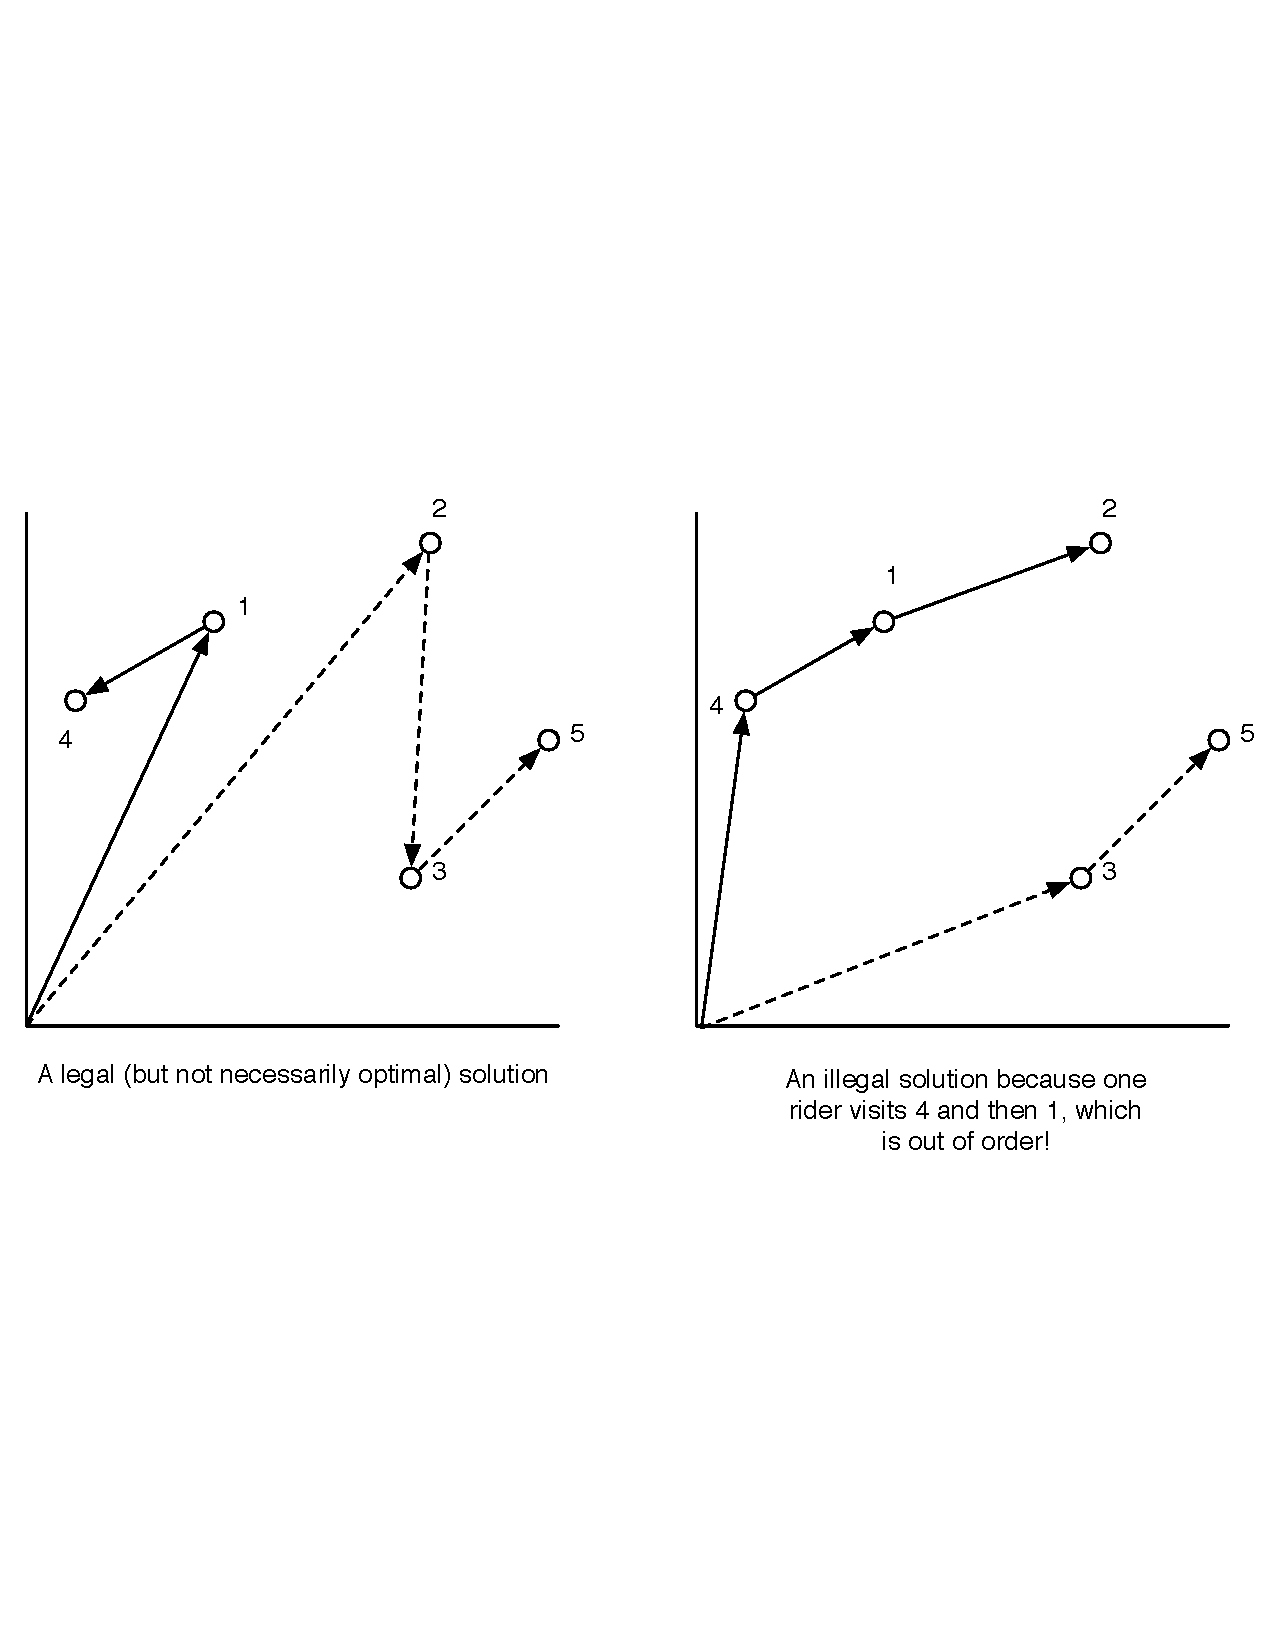
\includegraphics[height=2in]{WheelDeliver.pdf}
    \caption{Two examples of routes for the two riders.  The origin denotes the starting point $p_0$.  One rider's route is shown with solid lines and the other with dashed lines.  The route on the left is fair because points are visited by increasing indices.  The route on the right is not fair because, for example, point $p_4$  is visited before point $p_1$.}
  \end{figure}

  Julie and Daphne have hired you to design an efficient algorithm that takes as input an array of points $P = (p_1,p_2,\dots, p_n)$, sorted by the times in which their orders arrived, and outputs the sequences of delivery points for the two riders.

  \begin{parts}
      \bonuspart[4] Derive a recurrence relation, including base case(s), that is suitable for an efficient dynamic-programming solution for this problem.
      Briefly justify its correctness.
      
      \begin{solution}
          
      \end{solution}
      
      \bonuspart[4] Give a (bottom-up) dynamic programming algorithm, including pseudocode, for this problem that has running time $O(n^2)$.
      
      \begin{solution}
          
      \end{solution}
  \end{parts}

\end{questions}

\end{document}